\section{PID}

\begin{frame}{Wielowymiarowy PID}
Schemat projektowania wielowymiarwego algorytmu PID:
\begin{itemize}
    \item Wyznaczenie odpowiedzi skokowych wszystkich torów
    \item Przyporządkowanie najbardziej znaczącym sygnałów sterujących do wyjść
    \item Strojenie poszczególnych regulatorów
\end{itemize}
Niektóre sygnały sterujące nie będą miały wpływu na sygnały wyjściowe. 
\end{frame}


\begin{frame}{Wielowymiarowy PID}
Wyznaczenie odpowiedzi skokowych dla wszystkich torów procesu:
	\begin{center}
		\begin{figure}[H]
            		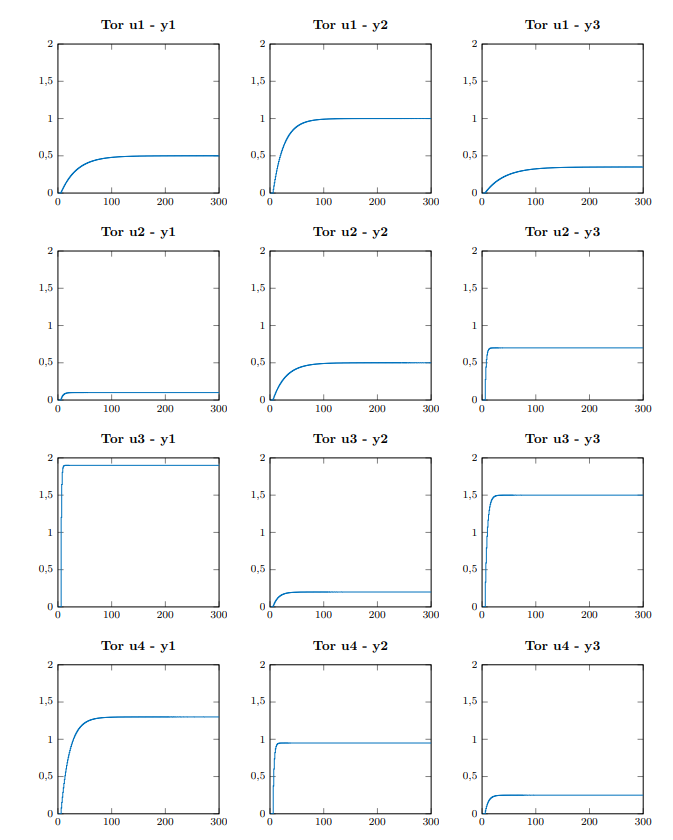
\includegraphics[scale=0.25]{images/PIDtory.png}
          			 \caption{Odpowiedzi poszczególnych torów dla skoku jednostkowego}
		\end{figure}
	\end{center}
\end{frame}

\begin{frame}{Wielowymiarowy PID}
Określenie pętli regulacji:
	\begin{center}
		\begin{figure}[H]
            		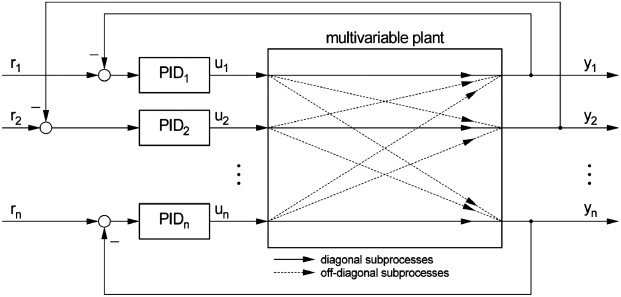
\includegraphics[scale=0.7]{images/MPID.jpg}
          			 \caption{Schemat układu regulacji}
		\end{figure}
	\end{center}
\end{frame}

\begin{frame}{Wielowymiarowy PID}
Wyniki działania:
	\begin{center}
		\begin{figure}[H]
            		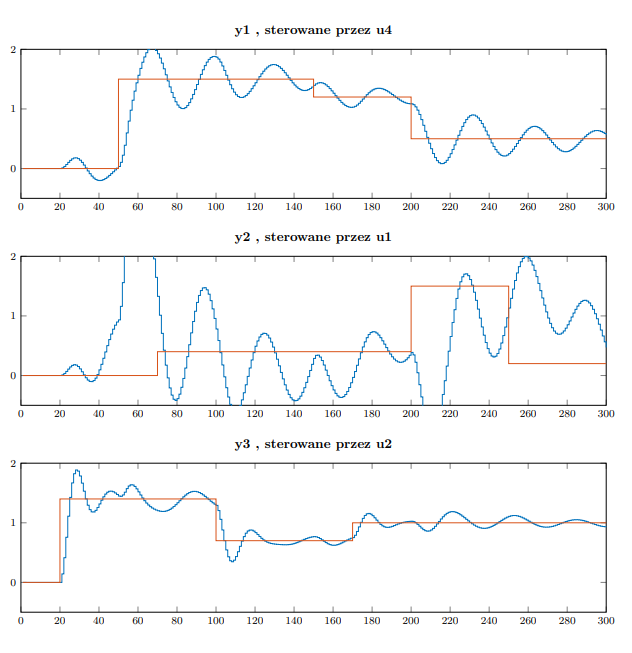
\includegraphics[scale=0.4]{images/MIMO_PID.png} %%do poprawy jak już będą ładne
          			 \caption{Wyniki regulacji}
		\end{figure}
	\end{center}
\end{frame}

